\section{Data Collection}

\begin{figure}[t]
\centering
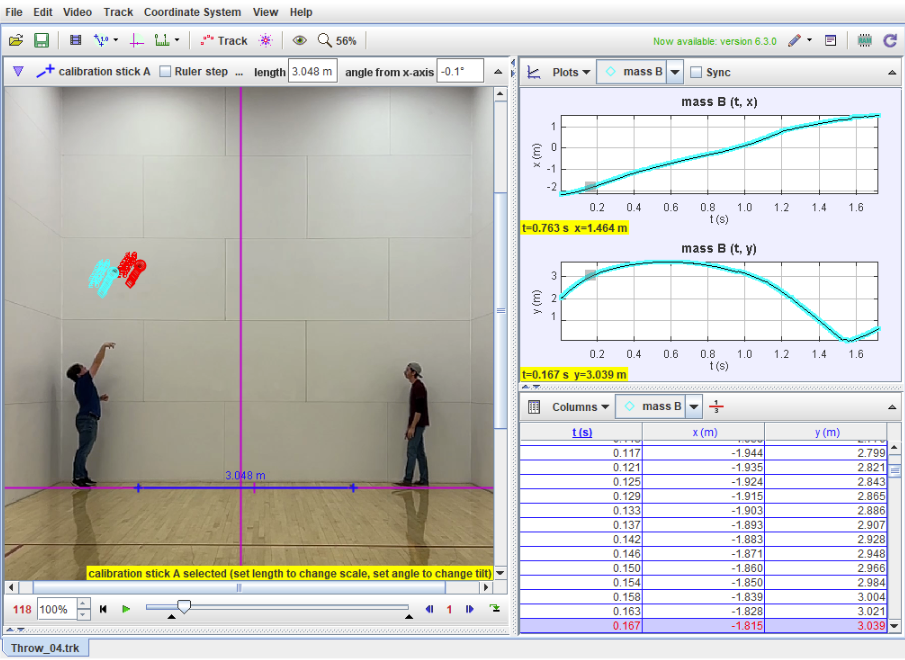
\includegraphics[width=.9\linewidth]{images/TrackerScreenshot.png}
\caption{\label{fig:TrackerScreenshot} Tracker being used to extract timestamped and calibrated position information from the video. Calibration is done by specifying the distance between two pixels, which we marked and measured with tape on the ground.}
\end{figure}

	Our data collection procedure was rather simple as increasing the complexity for this section would introduce more potential sources of error. We first found a location with good lighting and a consistent background, the location that we chose was one of the racquetball courts on campus. 
	
	Next using a tripod we set up our camera making sure to have a clear view of the projectiles trajectory ensuring that that the projectile was always in frame. This was done so that Tracker could extract the data points modeling the projectiles path. Once this was completed multiple trials were attempted being as consistent as possible. 
	
	In order to incorporate variable drag multiple chute designs were implemented. This was completed so that we could test the viability of our codes ability to model drag and its effect on trajectory. 
	
	One hour of video was collected, and a small portion of the videos were then processed in Tracker to be analyzed by our MATLAB script. Fig.~\ref{fig:TrackerScreenshot} shows what it looks like to use Tracker.